\chapter{L’intelligence artificielle et ses composantes}
\section{Introduction}
L’industrie représente l’un des terreaux les plus fertiles pour l’intelligence artificielle, vue  l’amélioration de la compétitivité qu'apporte l’intelligence artificielle à l’industrie. En lui offrant plusieurs avantages particulièrement  . l’entreprise peut organiser sa chaîne logistique, maîtriser  les données et les flux, facilite l’analyse des paramètres qui influencent la performance d’une ligne de production,et, permettent de faire des propositions d’optimisation des procédés de production. 

Autre atout de l’intelligence artificielle descriptive est qu’elle permet de distinguer quelles sont les tâches pouvant être améliorées, et les autres. Intégrée aux machines et logiciels de planification, elle identifie les tâches répétitives à faible valeur ajoutée qui peuvent être automatisées et donc prises en charge par des systèmes intelligents. 

Dans la suite de ce chapitre, nous allons définir l'intelligence artificielle et toutes les notions incluses dans ce vaste concept, nous donnerons des explications mathématiques et informatiques dans des points critiques tels que le Deep Learning qui est une sous-famille de Machine Learning qui est lui-même inclus dans l'IA, la figure suivante illustre le positionnement des mots clés dans ce chapitre


\begin{figure}[h]
    \centering
    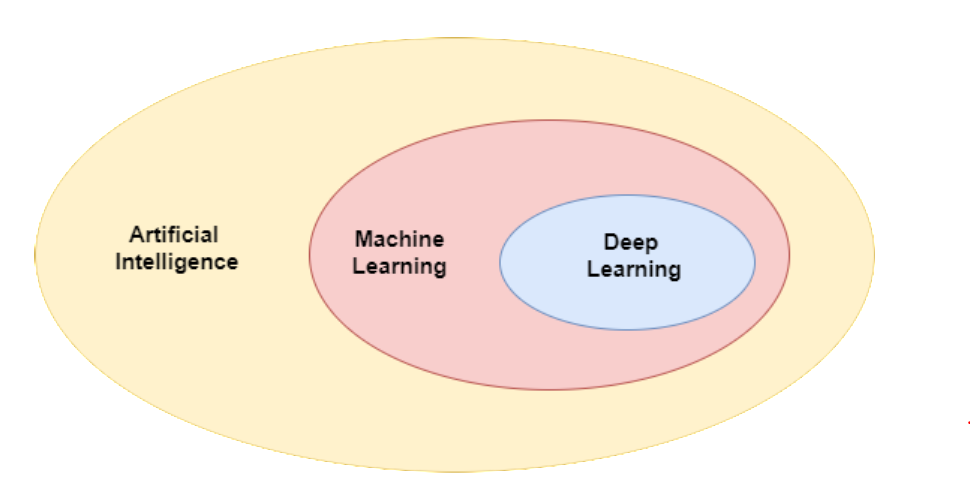
\includegraphics[width=10cm]{assets/PartOne/Chaptertwo/relationentreintelligenceartificielleetmachinelearningetdeeplearning.png}
    \caption{La relation entre l'intelligence artificielle, machine learning et deep learning}
    \label{relationentreintelligenceartificielleetmachinelearningetdeeplearning}
    \end{figure}

\newpage

\section{Intelligence artificielle}
\subsection{Définitions de l’intelligence artificielle}
La définition de l'intelligence artificielle a traversé de nombreuses définitions au fil des ans, et à ce jour il n'y a pas de définition officielle pour ce concept. Par exemple Asa B.Simmons et Steven G. Chappell \cite{simmonsArtificialIntelligencedefinitionPractice1988} ont défini le terme "intelligence artificielle" comme le comportement d'une machine qui, si un humain se comporte de la même manière, alors cette machine est considérée comme intelligente. Il est difficile d'étendre cette définition car la définition des facteurs qui décrivent l'intelligence humaine n'est pas claire.

Il existe une autre définition qui rend compte de la nature du travail effectué dans le domaine technologique. Elle a été proposée par E. Rich \cite{richArtificialIntelligenceHumanities1985} et se lit comme suit : ”L'intelligence artificielle est l'étude qui consiste à faire aux ordinateurs des choses que, pour l'instant, les humains font mieux.” Cette définition semble simple, mais critique en même temps, car il peut y avoir actuellement des machines qui surpassent les humains, par exemple, les systèmes prédictifs qui peuvent nous donner des résultats auxquels les gens ne pensent pas à travers les calculs complexes qu'ils effectuent.

Donc, comme nous l'avons déjà dit “L’intelligence artificielle” (IA) est une notion paradoxale car, comme le souligne Yoshua Bengio, on ne rend pas l’ordinateur plus intelligent mais on le rend au contraire moins stupide. Et on peut dire que L’IA est à la fois une discipline de recherche et une matière, à l’instar des mathématiques ou de la physique, utilisée dans de nombreuses autres disciplines de recherche, comme la médecine\cite{WillMachinesEliminate}.

Aujourd'hui plus que jamais, comprendre ce qu'est l'IA, ce qu'elle fait, ce qu'elle fera sûrement et ce qu'elle ne fera certainement jamais est un moyen ingénieux de comprendre et d'anticiper, même partiellement, le champ des possibles, et donc de s'y préparer, en tirant tous les bénéfices tout en écartant les éventuelles menaces.

Pour cela et en termes de définition simple, On peut définir l’IA comme l'intelligence artificielle est la capacité d'une machine ou d'un dispositif informatique à imiter l'intelligence humaine (processus cognitif), à acquérir des expériences, à s'adapter aux dernières informations et à réaliser des activités semblables à celles des humains\cite{klagesPatchBasedGenerative2019}.

\subsection{Typologie de l’intelligence artificielle}
Selon \cite{QuEstceQuea} l’IA peut être classée comme faible ou forte. L’IA faible, ou IA étroite, est un système d’intelligence artificielle conçu et entraîné pour une tâche particulière. Ainsi, les assistants personnels virtuels comme Siri d’Apple, sont une forme d’IA faible. Quant à l’IA forte, ou intelligence générale artificielle, elle dispose de capacités cognitives humaines.

\subsubsection{L’intelligence artificielle forte}
La définition de l’intelligence artificielle forte correspond à une intelligence pouvant remplacer intégralement l’étendue de l’intelligence humaine, dans toute sa complexité. Cette approche universelle d’un homme-machine existe depuis les Lumières, mais demeure un fantasme de nos jours.

Plusieurs dimensions de l’intelligence appartiennent à l’intelligence artificielle forte : parmi elles on compte les intelligences cognitives, psychomotrices, sociales et émotionnelles. La plupart des programmes contemporains intégrant l’AI fait essentiellement appel à l’intelligence cognitive : logique, organisation, résolution de problèmes, autonomie ou formation d’une perspective individuelle.

\subsubsection{L’intelligence artificielle faible}
L’intelligence artificielle faible, à l’inverse, se définit par le développement et l’utilisation de l’intelligence artificielle uniquement dans des domaines d’applications définis et limités. Les recherches sur l’AI en sont actuellement à ce stade, dans la mesure où ses champs d’application sont restreints à des domaines « faibles » mais hautement spécialisés : voitures autonomes, diagnostics médicaux, algorithmes de recherche, etc.

La recherche a fait des progrès considérables dans le domaine de l’IA faible. Le développement de systèmes intelligents dans des domaines spécifiques s’est avéré non seulement plus pratique, mais également plus éthique que les recherches sur la super intelligence. Les aires d’application de l’intelligence artificielle faible sont très vastes, mais réussissent particulièrement bien dans la médecine, la finance, les transports, le marketing, et évidemment Internet. On peut déjà prévoir que des technologies d’intelligence artificielle de ce type vont prendre de plus en plus d’importance dans presque tous les domaines de la vie quotidienne.

\section{L’apprentissage Automatique (Machine Learning)}
L'apprentissage automatique ou le machine Learning (ML) est la science et l'art de la programmation des ordinateurs afin qu'ils puissent apprendre des données.

Voici une définition un peu plus générale :

"L'apprentissage automatique est le domaine d'étude qui donne aux ordinateurs la capacité d'apprendre sans être explicitement programmé”\cite{samuelStudiesMachineLearning1988}.

Et une autre plus axé sur l'ingénierie :

On dit qu'un programme informatique apprend de l'expérience E par rapport à une tâche T et une certaine mesure de performance P, si sa performance sur T, mesurée par P, s'améliore avec l'expérience \cite{strachanWorldwideVariationsPrevalence1997}.

Par exemple, un filtre anti-spam est un programme d'apprentissage automatique qui peut apprendre à signaler les spams en donnant des exemples de spams (signalés par les utilisateurs, par exemple) et des exemples de courriels normaux (sans spams). Les exemples que le système utilise pour apprendre sont appelés l'ensemble d'apprentissage. Chaque exemple d'apprentissage est appelé instance d'apprentissage (ou échantillon).

Dans ce cas, la tâche T est de signaler le spam pour les nouveaux emails, l'expérience E est la formation donnée, et la mesure de performance P doit être définie ; par exemple, on peut utiliser le ratio d'e-mails correctement classés. Cette mesure de performance particulière est appelée précision et est souvent utilisée dans les tâches de classification.
\newpage
\subsection{Types d'Apprentissage Automatique}
Selon \cite{book} Il existe tellement de types différents de systèmes d'apprentissage automatique qu'il est utile de les classer en grandes catégories basées sur :
\begin{itemize}
    \item Qu'ils soient formés ou non sous supervision humaine (supervisé, non supervisé, semi-supervisé et apprentissage par renforcement)
    \item S'ils peuvent ou non apprendre progressivement en ligne ou hors ligne (apprentissage en ligne ou apprentissage par lots)
    \item Qu'ils fonctionnent simplement en comparant de nouveaux points de données à des points de données connus, ou à la place en détectant des modèles dans les données d'entraînement et en construisant un modèle prédictif (apprentissage basé sur des instances ou apprentissage basé sur des modèles)
    
\end{itemize}

Ces critères ne sont pas exclusifs, nous pouvons les combiner comme nous le souhaitons. Par exemple, un filtre anti-spam à la pointe de la technologie peut apprendre en ligne à l'aide d'un modèle de réseau neuronal profond formé à l'aide d'exemples de spam et de non-spam, cela en fait un système d'apprentissage supervisé en ligne basé sur des modèles.

Nous examinerons chacun de ces critères ci-dessous :
\subsubsection{Apprentissage Supervisé/Non Supervisé }
Les systèmes d'apprentissage automatique peuvent être classés en fonction de la quantité et du type de supervision qu'ils reçoivent pendant l'entraînement \cite{book}. Il existe quatre grandes catégories : l'apprentissage supervisé, l'apprentissage non supervisé, l'apprentissage semi-supervisé et l'apprentissage par renforcement.

\paragraph{Apprentissage supervisé}

Dans l'apprentissage supervisé, les données d'entraînement qu’on transmet à l'algorithme incluent les solutions souhaitées, appelées étiquettes. La Figure \ref{apprentissagesupervisé} montre exemple d’un ensemble d'entraînement étiqueté pour l’apprentissage supervisé.

\begin{figure}[h]
    \centering
    \includegraphics[width=10.5cm]{assets/PartOne/Chaptertwo/apprentissagesupervisé.png}
    \caption{Exemple d’un ensemble d'entraînement étiqueté pour l’apprentissage supervisé}
    \label{apprentissagesupervisé}
    \end{figure}

    
\newpage
Deux types d'algorithmes sont utilisés dans l'apprentissage supervisé : la classification et la régression. La classification est utilisée pour répondre à la question "Quelles classes ? ", tandis que la régression est utilisée pour répondre à la question "Combien ? “.

Ces deux approches comprennent une variété d'algorithmes. Certains de ces algorithmes peuvent être utilisés à la fois pour les problèmes de classification et de régression. Parmi des algorithmes d'apprentissage supervisé les plus importants :
\begin{itemize}
    \item La régression linéaire
    \item La régression logistique
    \item Le support vecteur machine
    
\end{itemize}

\paragraph{La régression linéaire :}
 
La régression linéaire est un algorithme ML utilisé pour l'apprentissage supervisé. La régression linéaire a pour but de prédire une variable dépendante (cible) en fonction de la ou des variables indépendantes données. Ainsi, cette technique de régression trouve une relation linéaire entre une variable dépendante et les autres variables indépendantes données \cite{RegressionAlgorithmsRegression2021}. La Figure \ref{régressinlinéaire} montre un graphe qui représente la régression linéaire.

\begin{figure}[h]
    \centering
    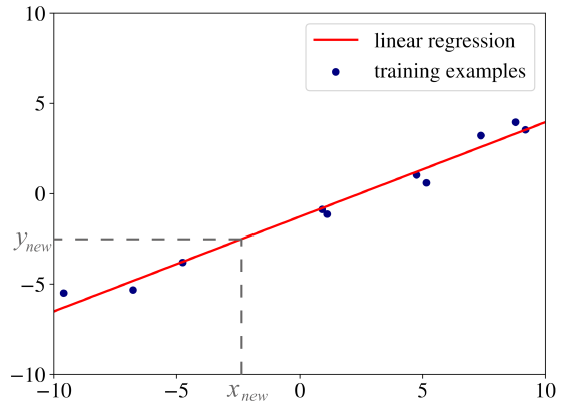
\includegraphics[width=12cm]{assets/PartOne/Chaptertwo/régressinlinéaire.png}
    \caption{Graphe représentant la régression linéaire}
    \label{régressinlinéaire}
    \end{figure}

    \newpage

\paragraph{La régression logistique :}
La régression logistique est un algorithme d'apprentissage automatique qui est utilisé pour les problèmes de classification, c'est un algorithme d'analyse prédictive basé sur le concept de probabilité. En effet, la régression logistique est un modèle linéaire généralisé qui utilise une fonction logistique comme une fonction de lien. La figure \ref{lafonctionlogistique} montre un graphe représentant la régression logistique : 

\begin{figure}[h]
    \centering
    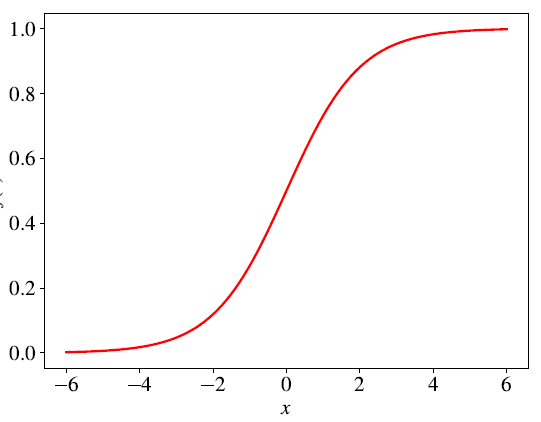
\includegraphics[width=10cm]{assets/PartOne/Chaptertwo/lafonctionlogistique.png}
    \caption{Graphe représentant la régression logistique}
    \label{lafonctionlogistique}
    \end{figure}


\paragraph{Le support vecteur machine : }
Cet algorithme utilise des hyperplans pour séparer les données. Dans le cas où cette séparation n'est pas possible, il utilise l'astuce du noyau où la dimension est augmentée et où les points de données deviennent séparables par un hyperplan \cite{RegressionAlgorithmsRegression2021}. La Figure \ref{supportvectormachine} montre un graphe représentant le support vecteur machine.


\begin{figure}[h]
    \centering
    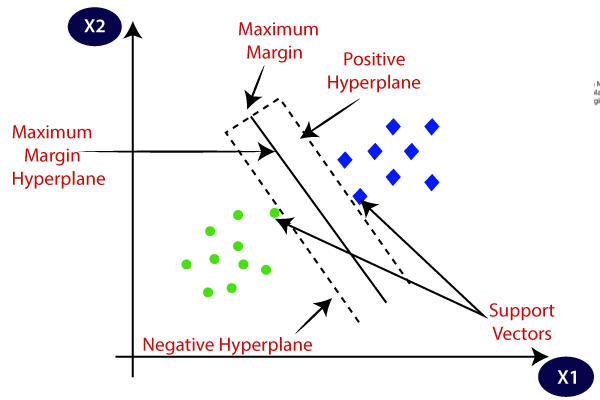
\includegraphics[width=10cm]{assets/PartOne/Chaptertwo/supportvectormachine.png}
    \caption{Graphe représentant le support vecteur machine}
    \label{supportvectormachine}
    \end{figure}

    \newpage

\paragraph{Apprentissage non supervisé}
Dans l'apprentissage non supervisé, les données d'apprentissage ne sont pas étiquetées. Le système essaie d'apprendre sans entrainement \cite{aggarwalNeuralNetworksDeep2018}. La Figure \ref{apprentissagenonsupervisé} montre exemple d’un ensemble d'entraînement non étiqueté pour l’apprentissage non supervisé.

\begin{figure}[h]
    \centering
    \includegraphics[width=10cm]{assets/PartOne/Chaptertwo/apprentissagenonsupervisé.png}
    \caption{Exemple d’un ensemble d'entraînement non étiqueté pour l’apprentissage non supervisé}
    \label{apprentissagenonsupervisé}
    \end{figure}

Ce type d’apprentissage contient aussi deux approches, le Clustering et l’Association. 

Le clustering est une méthode de regroupement des objets en clusters, de sorte que les objets présentant le plus de similitudes restent dans un groupe et ont moins ou pas de similitudes avec les objets d'un autre groupe. L'analyse par grappes trouve les points communs entre les objets de données et les catégorise en fonction de la présence ou de l'absence de ces points communs.

L’association est une méthode d'apprentissage non supervisée qui est utilisée pour trouver les relations entre les variables dans une grande base de données. Elle détermine l'ensemble des éléments qui se produisent ensemble dans l'ensemble de données. La règle d'association rend la stratégie de marketing plus efficace. Par exemple, les personnes qui achètent un article X (un pain, par exemple) ont également tendance à acheter un article Y (beurre/confiture). Un exemple typique de règle d'association est l'analyse du panier de la ménagère.

Puisque notre étude ne se concentre pas sur l'apprentissage non supervisé dans ce mémoire, on a pas détailler les algorithmes de ce type.

\paragraph{Apprentissage semi-supervisé}
L'apprentissage semi-supervisé est une classe de techniques d'apprentissage automatique qui utilise un ensemble de données étiquetées et non étiquetées. Il se situe ainsi entre l'apprentissage supervisé qui n'utilise que des données étiquetées et l'apprentissage non supervisé qui n'utilise que des données non étiquetées. Il a été démontré que l'utilisation de données non étiquetées, en combinaison avec des données étiquetées, permet d'améliorer significativement la qualité de l'apprentissage .
    